\section{SRv6}

IPv6 Segment Routing header: 
Next header field: 43 = Routing

\begin{itemize}
    \item \emph{Segment $\rightarrow$ IPv6 address}
    \item \emph{Segment list $\rightarrow$ Address list in the SRH}
\end{itemize}

A pointer in the SRH points to the Active Segment in the list of segments encoded in the header. No segments are removed while forwarding the packet, only pointers manipulated.
Active Segment is copied to the destination address field of the IP header.

\begin{itemize}
    \item Last segment index is 0
    \item First segment index is \emph{first segment}
    \item Active segment index is \emph{segments left}
\end{itemize}

\subsection{The SR Procedure}
If source node is SR capable, the following steps are applied to a packet:
\begin{enumerate}
    \item SR Header is created with the segment list in reversed order of the path.
    \item Segment list $[0]$ is the \emph{last} segment
    \item Segment list $[n-1]$ is the \emph{first} segment
    \item Segments left is set to $n-1$
    \item First segment is set to $n-1$
\end{enumerate}

In case a node in transit is not SR-enabled, plain IPv6 forwarding based on the Destination Address header field can be used. 
No inspection or update of the SR-header is performed.

This results in \emph{\textbf{full interoperability}} between SRv6 and IPv6 nodes.

\vspace{5mm}
\noindent
SR Segment Endpoints perform the following steps

\noindent
IF (segments left $>$ 0), THEN 
\begin{enumerate}
    \item Decrement Segments left by 1
    \item Update DA with Segment List [Segments left]
    \item Forward according to the new DA
\end{enumerate}

\noindent
ELSE (segments left = 0)
\begin{enumerate}
    \item Remove the IP and SR header
    \item Process the payload
    \begin{itemize}
        \item Inner IP: Lookup DA and forward
        \item TCP/UDP: send to socket
    \end{itemize}
\end{enumerate}

\emph{The final destination does not have to be SR-capable.}

\subsection{Segment format}
SRV6 SID is a 128-bit address.
Locator part routes to the node performing any possible function defined in the second part.

\emph{Optional}: the function part can be split into function bits and argument bits.
\begin{figure}[h]
    \centering
    
\includegraphics[width=7cm]{srv6-locator-function.png}
\end{figure}

\subsubsection{SRv6 uSID}
Combines several router IDs into one SRv6 SID. Completely compatible with default SRv6 SIDs.

\begin{figure}
    \centering
    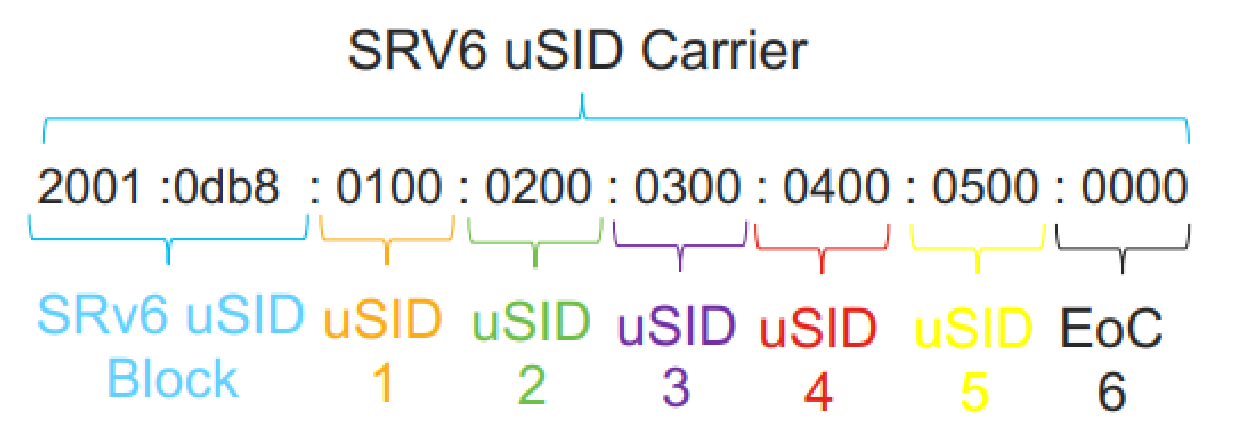
\includegraphics[width=8cm]{srv6-uSID.png}
\end{figure}

\vspace{5mm}
\noindent
SRv6 Locator is configured by device:

\ttfamily
\vspace{3mm}
\noindent
segment-Routing \\
\hspace*{1em}srv6\\
\hspace*{2em}locators\\
\hspace*{3em}locator MAIN\\
\hspace*{4em}micro-segment behavior unode psp-usd\\
\hspace*{4em}prefix fcbb:bb00:100::/48\\    
\rmfamily

\vspace{5mm}
\noindent
ISIS configuration for SRv6:

\ttfamily
\vspace{3mm}
\noindent
router isis 1\\
\hspace*{1em}address-family ipv6 unicast\\
\hspace*{2em}segment-routing srv6\\
\hspace*{3em}locator MAIN
\rmfamily

\vspace{5mm}
\noindent
BGP Control Plane: per-VRF oder per-CE modes possible

\ttfamily
\vspace{3mm}
\noindent
router bgp 1\\
\hspace*{1em}vrf 1\\
\hspace*{2em}address-family ipv4 unicast\\
\hspace*{3em}segment-routing srv6\\
\hspace*{4em}locator MAIN\\
\hspace*{4em}alloc mode per-vrf\\
\rmfamily